% Experiment 3: backend/evals/paper/exp3_reference.py   (30 seeds)
% Experiment 4: backend/evals/paper/exp4_store.py       (deterministic)
% Experiment 9: backend/evals/paper/exp9_normalize.py   (adversarial names)
\emph{Setup.} We simulated 16 weeks of claims for one item, a chicken puff with an
administrator reference of Rs.~20 and band Rs.~15--30, from 40 runners filing about
1.5 claims a week. Honest runners report Rs.~20, or Rs.~22 on the 15\% of days the
canteen charges more. Dishonest runners follow one of four strategies: \emph{line},
claiming 95\% of the allowance above the reference every time; \emph{evasive}, doing
so on a random half of their claims, intending to stay under the 60\% share the
near-line rule requires; \emph{overt}, claiming Rs.~30; and \emph{volume}, one runner
claiming at the line ten times as often as anyone else. The reference is
re-estimated weekly, and every claim is judged by the production code against the
reference in force when it was made. Each configuration was run with 30 seeds, and
we report the mean with the half-width of a 95\% confidence interval.

\begin{table*}[!t]
\caption{Reference Price (Rs.) After 16 Weeks, by Estimator and Attack.
Mean (95\% CI Half-Width) Over 30 Seeds}
\label{tab:reference}
\centering
\footnotesize
\setlength{\tabcolsep}{5pt}
\begin{tabular}{@{}lcccccc@{}}
\toprule
& \multicolumn{3}{c}{Line-walking} & Evasive & Overt & Volume \\
\cmidrule(lr){2-4}\cmidrule(lr){5-5}\cmidrule(lr){6-6}\cmidrule(l){7-7}
Dishonest runners & 30\% & 50\% & 60\% & 60\% & 60\% & 1 of 40 \\
\midrule
Mean, all claims & 24.14 (0.19) & 30.97 (0.40) & 37.80 (0.61) & 24.06 (0.18) & 26.06 (0.10) & 22.35 (0.12) \\
Mean, unflagged & 24.14 (0.19) & 30.97 (0.40) & 37.80 (0.61) & 24.06 (0.18) & 20.33 (0.02) & 22.35 (0.12) \\
Median, unflagged & 20.00 (0) & 31.27 (4.50) & 70.00 (0) & 20.00 (0) & 20.00 (0) & 20.00 (0) \\
One vote per runner & 20.00 (0) & 28.82 (0.97) & 96.96 (3.05) & 20.26 (0.26) & 20.00 (0) & 20.00 (0) \\
\quad + line-walkers excluded & 20.00 (0) & 20.00 (0) & 20.00 (0) & 20.00 (0) & 20.00 (0) & 20.00 (0) \\
\quad + band only & 20.00 (0) & 28.54 (0.91) & 27.50 (0.38) & 20.26 (0.26) & 20.00 (0) & 20.00 (0) \\
Deployed (both) & 20.00 (0) & 20.00 (0) & 20.00 (0) & 20.00 (0) & 20.00 (0) & 20.00 (0) \\
\bottomrule
\multicolumn{7}{@{}l@{}}{\scriptsize True price: Rs.~20, or Rs.~22 on dear days.
``(0)'' means every seed gave the same value.}
\end{tabular}
\end{table*}

\emph{The reference.} Table~\ref{tab:reference} shows three defences doing three
different jobs. Excluding flagged claims stops overt inflation: the mean of all claims
rose to Rs.~26.06 because flagged claims kept voting, while the mean of unflagged
claims stayed near the true price. One vote per runner stops volume: a single runner
filing ten times as often moved either mean by 12\% and no median at all. Against
line-walking, whose claims are never flagged, the vote limit is not enough on its
own. The median-based estimators held with 30\% dishonest runners and broke at 50\%,
and the one-vote estimator, whose allowance grows with the reference, ran away to
Rs.~96.96 at 60\% (Fig.~\ref{fig:reference}). The band bounded that drift. What held
the reference at Rs.~20 in every one of the 30 seeds was the exclusion of runners
under a near-line flag. Across all 4,620 runs no honest runner received a near-line
flag and no honest claim was judged FLAGGED.

\begin{figure}[!t]
\centering
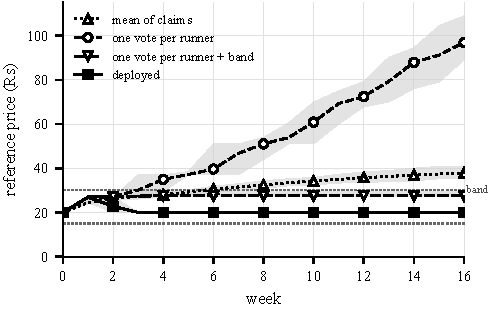
\includegraphics[width=\columnwidth]{figures/fig_reference.pdf}
\caption{Reference price week by week with 60\% of runners line-walking. Lines are
the mean over 30 seeds; shaded bands span the 5th to 95th percentile of seeds. The
deployed estimator rises while the near-line rule is still collecting four claims
from each attacker, then returns to the true price once their votes are excluded.}
\label{fig:reference}
\end{figure}

\emph{Why most evasive attackers were caught.} An evasive attacker inflates half of
their claims, so their long-run share of near-line claims is 0.50, and only 15--19\%
of them ever reached 60\% over their whole history. Yet 79--85\% were flagged. The
reason is in how the rule is evaluated, not in its threshold. It runs after every
claim, over the last 30 days, which for these runners holds about six judged claims.
With six fair coin flips, four or more heads has probability $22/64\approx0.34$, and
the rule gets a fresh chance at every submission. At the moment of flagging, the
window held on average 6.4 claims, of which 4.5 were near the line, a share of 0.72.
An attacker who wants to stay clear has to keep the \emph{windowed} share under 60\%,
which at this claim rate means inflating well under half the time.

\begin{table}[!t]
\caption{Money and Time to Detection Under the Deployed Estimator.
Mean (95\% CI Half-Width) Over 30 Seeds}
\label{tab:money}
\centering
\scriptsize
\setlength{\tabcolsep}{2.4pt}
\begin{tabular}{@{}lccccc@{}}
\toprule
& & Attackers & Days to & \multicolumn{2}{c}{Excess paid (Rs.)} \\
\cmidrule(l){5-6}
Strategy & Attackers & flagged & first flag & before flag & 16 weeks \\
\midrule
Line, 10\% & 4 & 100\% & 19.1 (2.0) & 110 (3) & 632 (20) \\
Line, 30\% & 12 & 100\% & 19.3 (1.2) & 331 (4) & 1958 (46) \\
Line, 60\% & 24 & 100\% & 19.0 (0.8) & 1016 (33) & 4370 (74) \\
Evasive, 10\% & 4 & 85\% & 48.0 (5.6) & 170 (12) & 316 (13) \\
Evasive, 30\% & 12 & 79\% & 46.4 (3.2) & 520 (21) & 954 (32) \\
Evasive, 60\% & 24 & 83\% & 45.3 (2.1) & 1019 (32) & 1986 (44) \\
Volume, 1 runner & 1 & 100\% & 3.8 (0.7) & 27 (1) & 1591 (46) \\
Overt, 60\% & 24 & n/a & n/a & $-167$ (8) & $-167$ (8) \\
\bottomrule
\multicolumn{6}{@{}p{0.97\columnwidth}@{}}{Excess paid is reimbursement above the
true price, summed over all attackers. ``Before flag'' counts claims made before each
attacker's first near-line flag; ``16 weeks'' assumes nobody reviews the flag.
Overt claims are flagged one by one and reimbursed at the reference, so overt
attackers recover less than they spend.}
\end{tabular}
\end{table}

\emph{Money and time.} Table~\ref{tab:money} reports what the attacks cost. The
near-line flag withholds nothing, by design, so the money only stops when an
administrator acts on it. Line-walkers were flagged after about 19 days, having
taken about Rs.~28 each by then. Evasive attackers who were flagged took about 46
days to reach it; counting the ones never flagged over their whole run, evasive
attackers took about Rs.~43 each outside any flag. The 16-week column is what the platform would pay if nobody
reviewed the flags. At 30\% line-walkers it is Rs.~1,958, about Rs.~7 per inflated
claim, which is why review capacity is part of the defence.

\emph{Names.} Binding a claim to the order's lines
(Section~\ref{sec:design-claims}) was tested with 61 names a runner might type for
three priced lines: misspellings, padded names (``chicken puff special''), obfuscated
ones (``ch1cken puff'', a Cyrillic letter, spaced letters), unrelated renames
(``snack'', ``zzq special''), and swaps to the name of an unpriced line on the same
order. Under the earlier rule, which matched names against the whole campus list, 41
of the 61 were paid unchecked. Under the deployed rule 20 are judged against the
right reference, 35 are refused, and none is judged against the wrong one. The six
that remain unchecked are the swaps. A runner can claim a priced item's money under
the name of a hand-typed, unpriced line on the same order, and that line has no
reference to judge it by. This is the cold-start case, and its bound is the escrow
hold: a payout above the hold freezes for review (Section~\ref{sec:eval-dispatch}).
The deterministic and fuzzy tiers also mapped 193 of 200 hand-written misspellings of
20 canteen items to the right key, none to a wrong one, and merged none of 20
look-alike items (``egg roll'', ``paneer tikka roll'') into a listed one. We wrote
all of these names ourselves, so the numbers measure coverage of the errors we
anticipated, not accuracy in the field.

\emph{Shops.} For shop-level pooling the same item was placed at a canteen charging
the reference and at dearer ones. Against the campus reference every honest claim at
a dearer counter is judged against Rs.~20, so an honest Rs.~30 claim is flagged and
Rs.~10 withheld for telling the truth. Table~\ref{tab:store}(a) shows when
\eqref{eq:store} has moved the shop's reference far enough. A shop charging Rs.~30
needs three distinct reporting runners and one charging Rs.~40 needs ten. A shop
charging Rs.~60 never gets there, because the drift cap holds its reference at
Rs.~50; such an item needs an administrator to list it separately. The same mechanism
is the weak point, and Table~\ref{tab:store}(b) measures it. The number of claims per
colluder made no difference at 1, 10 or 50, because each runner has one vote. The
number of colluders did. At a shop with few honest reporters, two or three colluders
claiming Rs.~30 were paid in full, Rs.~10 above the true price per claim; with ten or
twenty honest reporters they had to match them in number. Every colluding claim in
the Rs.~30 rows still counted toward the walking-the-line rule, which is judged
against the shop-adjusted reference, so colluders who keep doing it are flagged as
line-walkers after four claims. Seeding the shop is not free either: until three
distinct runners have reported there, each colluder's Rs.~30 claim is judged against
Rs.~20 and flagged, which counts toward the strike ladder.

\begin{table}[!t]
\caption{Shop-Level Pooling Against a Campus Reference of Rs.~20}
\label{tab:store}
\centering
\scriptsize
\setlength{\tabcolsep}{3pt}
\begin{tabular}{@{}cccc@{}}
\toprule
\multicolumn{4}{@{}l}{(a) Distinct honest reporters before an honest claim is paid in full} \\
Shop price & Reporters needed & Shop reference then & Withheld before \\
\midrule
Rs.~25 & 0 & 20.00 & 0 (within allowance) \\
Rs.~30 & 3 & 23.33 & Rs.~10 \\
Rs.~40 & 10 & 32.50 & Rs.~20 \\
Rs.~60 & never (cap Rs.~50) & 50.00 & Rs.~10 at 20 reporters \\
\midrule
\multicolumn{4}{@{}l}{(b) Colluders needed to be paid in full at a Rs.~20 shop} \\
Honest reporters & Claiming Rs.~30 & Claiming Rs.~40 & Claiming Rs.~50 \\
\midrule
0 & 3 & 10 & 20 \\
1 & 2 & 8 & 20 \\
3 & 3 & 8 & 15 \\
5 & 5 & 8 & 15 \\
10 & 10 & 11 & 11 \\
20 & 20 & $>$20 & $>$20 \\
\bottomrule
\multicolumn{4}{@{}p{0.95\columnwidth}@{}}{Every colluder files 1, 10 or 50 claims;
the counts are identical in all three cases. Honest reporters each claim Rs.~20
twice.}
\end{tabular}
\end{table}
